\chapter{random variable}

\begin{definition}{random variable}
    对于 probability space \((\Omega, \mathcal{F}, \mathbb{P})\), 一个 random variable 是一个 \textbf{Borel measurable function} $X: \Omega \rightarrow \mathbb{R}$.
\end{definition}

\begin{remark}
    回顾 measurable function 的定义: 即对于任意 Borel set $B \subset \mathbb{R}$, 有 $X^{-1}(B) \in \mathcal{F}$.
    例如: \(X(\omega) = \omega^2\) 是一个 measurable function, 因为对于任意 Borel set $B \subset \mathbb{R}$, 有 $X^{-1}(B) = \{\omega \in \Omega | \omega^2 \in B\} \in \mathcal{F}$.
\end{remark}


% 其 cdf $F_X: \mathbb{R} \rightarrow [0,1]$ 就是 $X$ 这个 real-valued measurable function 对于 $(-\infty,x]$ 的 preimage, 意义是 "随机变量的值小于等于 $x$ 的概率"  
% \[
% F_X (x) = P( X^{-1}(-\infty,x))
% \]
% discrete random variable 的 pmf, 表示每个离散点 $x$ 的 $P(X^{-1}(\{x\}))$.
% 即 \[
% p(x) := P(X^{-1}(\{x\})) = P(X=x)
% \]
% continuous random variable 的 pdf, 表示在某个点上概率分布的密度有多大 \[
% f_X(x) :=  \frac{dF_X(x)}{dx}
% \]
% 或者写作: \[
% f_X(x) :=  \frac{dF_X(x)}{dm}
% \]
% 是这个 $F_X$ 对于 Lebesgue measure $m$ 的 Radon-Nikodym derivative.



\begin{proposition}
    Prob space \((\Omega, \mathcal{F}, \mathbb{P})\) 上的 
    random variables \(X_1, X_2, \ldots, X_k: \Omega \rightarrow \mathbb{R}\),
    任取 Borel measurable function \(g: \mathbb{R}^k \rightarrow \mathbb{R}\), 
    \begin{align*}
        X: \Omega &\rightarrow \mathbb{R} \\
        \omega &\mapsto g(X_1(\omega), X_2(\omega), \ldots, X_k(\omega))
    \end{align*}
    也是一个 random variable.
\end{proposition}
\begin{proof}
    我们在 measure theory 中证明过: 对于任意的 finite seq of Borel measureable functions 
    \( (  {f_i}: \Omega \to \mathbb{R} )_{i=1}^k\), 其各作为一个维度组成的函数
    \(f = (f_1,\cdots, f_k)\) 也是一个 Borel measurable function (from \(\Omega\) 到 \(\mathbb{R}^k\)).\\
    而这里的 \(X\) 就是 \(g \circ f\), 是两个 Borel measurable function 的 composition, 因而也是一个 Borel measurable function (即 random variable).
\end{proof}
\begin{remark}
    以一种 Borel measurable 的方式组合多个 random variables, 这个函数也仍然是一个 random variable.
\end{remark}


\section{distributions}
\subsection{distribution and cumulative distribution function}
\begin{definition}{probability distribution}
    对于 random variable \(X: \Omega \to \mathbb{R}\) on \(\Omega, \mathcal{F}, \mathbb{P}\), 
    其 probability distribution 是 \(X\) 对于 \(\mathbb{P}\) 的 pushforward measure, 
    记作 \(\bP^X: \mathcal{B}(\mathbb{R}) \to [0,1]\). 即
    \[
    \bP^X(B) := \bP(X^{-1}(B)), \quad \forall B \in \mathcal{B}(\mathbb{R})
    \]
    我们 write:
    \[
    X \sim \bP^X
    \]
\end{definition}
\begin{remark}
    看着有点不直观. 实则我们拆解:
    \begin{itemize}
        \item \(X^{-1}(B)\) 即: 有多少 samples (即哪一个事件 \(E\in\mathcal{F}\)) 在这个 RV $X$ 的映射下落入 \(B\) 这个区间?
        \item \(\bP(X^{-1}(B))\) 即: 这个事件 \(E\) 的概率是多少?
    \end{itemize}
    接下来的定义和例子会更加直观.
\end{remark}
\begin{definition}{distribution function (也称 \textbf{cumulative distribution function, cdf})}
    对于 random variable \(X: \Omega \to \mathbb{R}\), 
    其 \textbf{cumulative distribution function} 是 \(\bP^X\) 这一函数的 distribution function, 
    记作 \(F_X\). 即对于任意 \(x \in \mathbb{R}\), 有
    \[
    F_X(x) := \bP^X((-\infty,x]) = \bP(X^{-1}((-\infty,x]))
    \]
\end{definition}
\begin{remark}
    \(F_X(x)\) 即 \(\bP(\{X\leq x\})\) 我们也会简写为 \(\bP(X \leq x)\).\\
    \(F_X(x)\) 的意义是: random variable \(X\) 的值不超过 \(x\) 的概率.\\
\end{remark}


\begin{example}{(geometric probability)}
Fix \(a,b >0\). 
我们在正方形区域 \(\Omega = [0,a] \times [0,b]\) 上均匀地随机选取一个点 \((x,y)\).\\
我们 define 随机变量: \(X: \Omega \to \bR\) by \(X(x,y) = x\). 求 \(X\) 的 distribution function \(F_X\).\\
这很简单: 对于 \(x\in [0,a]\),
\[
F_X(x) = \bP(X \leq x) = \frac{m([0,x]\times [0,b])}{m([0,a]\times [0,b])} = 
\frac{x \cdot b}{a \cdot b} = \frac{x}{a}, \quad 0 \le x \le a
\]
因为
\begin{equation}
    F_X(x) = \begin{cases}
    0, & x < 0 \\
    \frac{x}{a}, & 0 \le x \le a \\
    1, & x > a
    \end{cases}
\end{equation}
注意: 在这个例子中, probability measure \(P\) 是 Lebesgue measure on \([0,a]\times [0,b]\). 很多时候我们在
计算 RV 的 distribution function 的时候, 都是直接直观地计算 \(P(X \leq x)\). 但是在稍微复杂一些
的例子中, 我们需要对各个条件的 formalization 更清楚一点.
\end{example}


\begin{theorem}{distribution function 的性质}\label{distribution function 的性质}
    对于 random variable \(X: \Omega \to \mathbb{R}\), 其 distribution function \(F_X\) 满足:
    \begin{itemize}
        \item \(F_X\) 是 non-decreasing (non-strictly increasing) 的.
        \item $\lim _{x \rightarrow+\infty} F_X(x)=1$, $\lim _{x \rightarrow-\infty} F_X(x)=0$.
        \item \(F_X\) 是 right-continuous 的. 即对于任意 \(x_0\), 有 \(\lim_{x \to x_0^+} F_X(x) = F_X(x_0)\).
        \item 对于任意 \(x_0\), 有 \(\lim_{x \to x_0^-} F_X(x) = P(X < x_0)\). 
        并且 \(\bP(X = x_0) = \lim_{x \to x_0^+} F_X(x) - \lim_{x \to x_0^-} F_X(x)\).
        \item 对于任意 \(x_1 < x_2\), 有 \(P(X \in (x_1,x_2]) = F_X(x_2) - F_X(x_1)\).
    \end{itemize}
\end{theorem}
\begin{proof}
    其他都显然. right-continuity 是源自 measure 的 continuity from above, 
    我们证明一下: 考虑一个单调递减序列 $\{x_n\}\downarrow x_0$, 
    令 seq of events \(A_n = \{X \leq x_n\}\), 注意这是一个嵌套递减的 set seq. 
    通过 \(\bR\) 的 completeness 容易证明:  \[A_0 = \bigcap_{n=1}^\infty A_n = \{\omega: X(\omega) \leq x_0\}\]
    由 measure 的 continuity from above, \(\bP(A_0) = \lim_{n\to\infty} \bP(A_n)\).
    也即 \(\lim_{x \to x_0^+} F_X(x) = \bP(X \leq x_0)\).\\
    而下面一条 \(\lim_{x \to x_0^-} F_X(x) = \bP(X < x_0)\) 同理是源自 measure 的
     continuity from below.\\
    那么 \(\bP(X = x_0) = \bP(X \leq x_0) - \bP(X < x_0)\) 是 natural 的 (by def).
\end{proof}

\begin{remark}
    我们此时心里会默认一件事情: 一旦知道了 RV \(X\) 的 distribution function 
    \(F_X\), 就知道了 \(X\) 的完整 distribution \(P^X\).
    这个直觉是对的. \\
    回忆一下: 我们在 measure theory 中, 
    证明 Carathéodory extension theorem 的时候, 
    证明过一个 \(\pi-\lambda\) theorem, 以它作为工具才
    把 premeasure 从一个 algebra extend 
    到一个 measure on the generated \(\sigma\)-algebra:
    \begin{theorem}{Dynkin's \(\pi-\lambda\) theorem}
        设 \(\mathcal{P}\) 是一个 \(\pi\)-system (closed under finite intersection), \(\mathcal{L}\) 是一个 \(\lambda\)-system 
        (closed under complementation and countable disjoint union), 
        如果 \(\mathcal{P} \subseteq \mathcal{L}\), 那么 \(\sigma(\mathcal{P}) \subseteq \mathcal{L}\).
    \end{theorem}
    
    我们考虑所有的 half-open interval \((-\infty,x]\) 组成的集合
     \(\mathcal{G}\), 这个集合 generate the Borel \(\sigma\)-algebra, 并且
     还是一个 \(\pi\)-system, 即: 它 closed under finite intersection:
     \[
     (-\infty, a] \cap (-\infty, b] \in \mathcal{G}, \quad \forall a,b \in \mathbb{R}
     \]
     然后考虑 \[
     \mathcal{L} := \{E \in \sigma(\mathcal{G}) : \bP_1(E) = \bP_2(E)\}
     \]
     即两个 measure 一致的 collection of sets.
     容易证明, 这个 \(\mathcal{L}\) 是一个 \(\lambda\)-system, 并且 \(\mathcal{G} \subset \mathcal{L}\).\\
     从而, \[\bB(\bR) =  \sigma(\mathcal{G}) \subseteq \mathcal{L}\] 并且 \(\bP_1(E) = \bP_2(E)\) 
     对于任意 \(E \in \bB(\bR)\).

     因而:
     \begin{corollary}{distribution function \(F_X\) determines distribution \(P^X\)}
         对于 random variable \(X: \Omega \to \mathbb{R}\), 其 distribution function \(F_X\) 确定了 distribution \(P^X\); 即
         如果两个 random variable \(X\) 和 \(Y\) 满足 \(F_X = F_Y\), 那么 \(\bP^X = \bP^Y\).
     \end{corollary}
\end{remark}


\subsection{discrete  random variable 与 probability mass function}
我们基本上研究两类 random variable: discrete random variable 和 continuous random variable.
\begin{definition}{discrete random variable}\label{discrete-rv}
    对于 random variable \(X: \Omega \to \mathbb{R}\),
     如果存在一个 countable set \(S \subseteq \mathbb{R}\) 
     使得 \(\bP(X \in S) = 1\), 
     那么 \(X\) 是一个 discrete random variable.
\end{definition}
\begin{remark}
    就是说, \textbf{\(X\) 的 range a.s. 是 countable 的} (允许 null set 上
    的值不在这个 countable set 里, 但是这是 measure theory 
    下的概念, 所以这些都可以忽略不计). 
\end{remark}
\begin{remark}
    对于 discrete random variable \(X\), 
    其 distribution function \(F_X\) 是一个 step function, 
    只有 countable 多个 jump discontinuity, 
    每个 jump 的大小就是 \(X\) 在那个点的 probability mass.\\
    因而, 对于 discrete random variable \(X\), 
    通常考虑其 \textbf{probability mass function (pmf)} \(p_X\) 更加有用:
    \begin{definition}{probability mass function (pmf)}
        对于 discrete random variable \(X\), 其 pmf 定义为
        \[
        p_X(x) := \bP(X = x), \quad \forall x \in \mathbb{R}
        \]
    \end{definition}
这个 pmf 就是 \(F_X\) 的 jump size function.
当然, 根据定义明显可得: \[
\sum_{x} p_X(x) = 1
\]
\end{remark}
 值得一提的是, 
    这个 \textbf{pmf 其实就是 \(X\) 的 distribution \(\bP^X\) 对于 counting measure (for range of \(X\))的 Radon-Nikodym derivative:}

\begin{proposition}{pmf 是 distribution 对于 counting measure \(\mu_S\) 的 Radon-Nikodym 导数}
对于一个 discrete random variable \(X\), 假设其 range 是 countable set \(S\), 
则我们定义 counting measure \(\mu_S\) on \(S\) 为: \[
\mu_S(A) := \sum_{x_i \in S} \mathbf{1}_A(x_i)
\]
那么, distribution \(\bP^X \ll \mu_S\) (绝对连续), 并且有:
     \[
     p_X = \frac{d\bP^X}{d\mu_{S}}
     \]
\end{proposition}
\begin{proof}
    这很容易证明. 首先, 这个 counting measure 即:
    \(A\) 中有多少个点在 \(S\) 中.\\
    那么显然, 如果 \(\mu_S(A) = 0\), 即 \(A\) 中没有点在 \(S\) 中, 
    那么 \(\bP^X(A) = 0\). 因而 \(\bP^X \ll \mu_S\).\\
    且对于任意 Borel set \(A\),
    \[
    \bP^X(A) = \sum_{x_i \in A} \bP(X = x_i) = \sum_{x_i \in A\cap S} p_X(x_i) = \int_A p_X(x) \;d\mu_{S}(x)
     \]  
\end{proof}

\subsection{continuous random variable 与 probability density function}
相对应 discrete random variable, 我们定义 continuous random variable:
\begin{definition}{continuous random variable}\label{continuous-rv}
    我们称一个 random variable \(X: \Omega \to \mathbb{R}\) 
    是一个 \textbf{continuous random variable}, 如果它的 cdf \(F_X\) 是一个 
     \textbf{absolutely continuous function.}
\end{definition}
\begin{remark}
    回顾 absolutely continuous function 的定义, 这是一个比较复杂的定义:
    对于任意 \(\epsilon > 0\), 都存在 \(\delta > 0\) 
    使得任取 finite collection of 
    disjoint intervals \(\{(a_i,b_i)\}\), 都满足: 
    \[\sum_i (b_i - a_i) < \delta \implies \sum_i |F_X(b_i) - F_X(a_i)| < \epsilon\]
    这是 uniform continuity 的一个加强版本. uniform continuity 对应的是 \(n=1\)
    的情况, 即: \textbf{任意的区间上, 只要长度足够小, 就能保证 \(F_X\) 在这个区间上的增量足够}小; 
     而 absolutely continuity 更严格: 
    \textbf{即便是任意数量的分散的区间, 只要总长度足够小, 就能保证 \(F_X\) 在这些 interval 上的增量的总和足够小.}

    这个定义有点麻烦, 不过存在等价的条件. 为此我们要 recall 一系列定义与结论, 详细请见: \href{https://qiulinfan.github.io/mathnotes-measure_theory/12-differentiation_on_real_spaces.html}{notes on measure theory, module 12: differentiation on \(\bR\)}:
    \begin{itemize}
        \item 给定一个 function \(F: \bR \to \bC\), 我们定义它的 
        \textbf{total variation function} \(V_F: \bR \to [0,+\infty]\) 为: \[
        T_F(x) := \sup \big\{ \sum_{i=1}^n |F(x_i) - F(x_{i-1}) \mid  -\infty < x_0 < \cdots < x_n \big\}
         \] \
        \item 如果 \(T_F(\infty)<\infty  \) (注意这是单调递增函数, 因而即对于任意的 \(x\) 都有 \(T_F(x) < \infty\)), 那么我们称 \(F\) 是一个 \textbf{function of bounded variation}, 写作 \(F \in BV\).
        \item 如果 \(F \in BV\), 且 \(F\) 是 right-continuous 的, 且 \(F(-\infty) = 0\), 那么我们称 \(F \in NBV\). (即 normalized function of bounded variation).
        \item \textbf{任意的 \(F \in NBV\) 都 \(m\)-a.e. differentiable, 且导数 \(F' \in L^1(m)\)}, 并且以下三个条件等价:
        \begin{align}
            &\quad\quad F \in AC  \\
            &\iff   \mu_F \ll m \\
            &\iff  F(x) = \int_{-\infty}^x F'(t) \;dt \quad\forall x \in \bR 
        \end{align}
    \end{itemize}
 \end{remark}

这几行字浓缩了 measure theory 的 differentiation theory 的两个星期的内容...
具体见上文 notes 链接, 都有详细证明.
而我们这里就利用起最后这一条结论. 首先, 我们 state 一件事:
\begin{lemma}{cdf 一定是 \(NBV\) 的} \label{cdf 一定是 NBV 的}
    任意的 random variable 的 cdf \(F_X\) 都是一个 \(NBV\) function.
\end{lemma}
\begin{proof}
    依旧见 notes, 有一个关键 lemma: \(F \in BV\) 当且仅当它可以表示为两个 
    monotone increasing function 的差. 
    而 random variable 的 cdf \(F_X\) 自身是一个 non-decreasing function, 因而首先 \(F_X \in BV\).\\
    其次, 由 \ref{distribution function 的性质} 我们知道, 
    \(F_X\) 是 right-continuous 的, 
    且 \(F_X(-\infty) = 0\). 因而 \(F_X \in NBV\).
\end{proof}
因而我们自然得出:
\begin{theorem}{一个 random variable 是 continuous random variable 的充要条件}
    一个 random variable \(X: \Omega \to \mathbb{R}\) 的 cdf 一定是 \(m\)-a.e.
     differentiable 的.\\
     \(X\) 是一个 continuous random variable 当且
    仅当 \(\bP^X \ll m\), 并且当且仅当 \[
    F_X(x) = \int_{-\infty}^x F'_X(t) \;dt \quad \forall x \in \bR
    \]
\end{theorem}
\begin{proof}
    即 remark 的最后一条结论. 由于 \(F_X\) 是一个 \(NBV\) function, 
    因而 \(F_X\) 是 \(m\)-a.e. differentiable 的.\\
    并且, \(F_X \in AC\) iff 它满足 FTC of Lebesgue integral.
    
\end{proof}
\begin{remark}
因而, 在简化的教材中, 通常会直接定义: 一个 random variable \(X\) 
是 continuous random variable, 
如果存在一个 \(f_X\) 使得 \(F_X(x) = \int_{-\infty}^x f(t)\;dt\) for all \(x\).
 这里其实是跳过了我们刚才的所有步骤, 直接使用了这个等价条件.
\end{remark}
\begin{remark}
    另外, 刚才还提到了另一个等价条件 \(\bP^X \ll m\), 
    即(by Radon-Nikodym theorem), 存在一个 radon-nikodym derivative \(f_X = \frac{d\bP^X}{dm}\) 
    使得对于任意 Borel set \(A\), 有 \[\bP^X(A) = \int_A f_X(x) \;dm(x)\]
    这其实和上面的 \(F_X(x) = \int_{-\infty}^x F'_X(t) \;dt\) 也是等价的.
    这里的 \(f_X\) 就是 \(F_X\) 的导数 \(F'_X\), 
    也就是我们通常说的 continuous random variable 的 \textbf{probability density function (pdf).}
\end{remark}

\begin{definition}{probability density function (pdf)}\label{probability density function}
    对于 continuous random variable \(X\), 其 probability density function 定义为 \(F_X\) 的 (\(m\)-a.e.)导数, 
    即
    \[
    f_X(x) := F'_X(x), \quad m\text{-a.e. } x \in \bR
    \]
\end{definition}
我们最后梳理一下.
\begin{itemize}
    \item \textbf{任意的 random variable} 的 cdf \(F_X\) 都是一个 \(NBV\) function, 因而\textbf{一定 a.e. 可导}.
     但是它的导数 \(F'_X\) 的积分不一定返回原函数.
    \item \textbf{如果一个 \(m\)-a.e. 导数 \(F'_X\) 满足 \(F_X(x) = \int_{-\infty}^x F'_X(t) \;dt\)
     对所有 \(x \in \bR\) 成立, 即导数的积分返回原函数, 那么 \(X\) 就是一个 continuous random variable}, 
     而我们定义 \(f_X := F'_X\) 为 \(X\) 的 probability density function.
\end{itemize}

以及, 显然 pdf 有以下性质:
\begin{proposition}{probability density function 的性质}
    对于 continuous random variable \(X\) with pdf \(f_X\), 
    \begin{itemize}
        \item \(f_X(x) \geq 0\) for \(m\)-a.e. \(x \in \bR\). (因为 \(F_X\) 是 non-decreasing 的.)
        \item \(\int_{-\infty}^{+\infty} f_X(x) \;dx = 1\). (因为 \(F_X(\infty) = 1\).)
        \item 对于任意 Borel set \(A\), 有 \[\bP(X\in A) =    \bP^X(A) = \int_A f_X(x) \;dx\]
        \item 对于 \(m\)-a.e. \(x \in \bR\), \[f_X(x) = \lim_{\epsilon \to 0^+} \frac{\bP^X([x, x+\epsilon))}{\epsilon} = 
        \lim_{\epsilon \to 0^+} \frac{F_X(x+\epsilon) - F_X(x)}{\epsilon}\]
    \end{itemize}
    
\end{proposition}

\subsection{singular continuous random variable 与 LDT 的应用}
对于 continuous random variable 的定义, 有些地方会简化定义为: continuous random variable 就是指其 cdf 是一个 continuous function.

但是我们现在知道, 这个定义是错的. 
首先, 标准定义中的 absolutely continuous 要强于 continuous (它能推导出 a.e. differentiable); 
而且, \textbf{这个更强的定义是 necessary 的}.

因为当提及 continuous random variable 时, 通常意思是它存在一个 pdf. 
而存在一个 pdf 即意味着它满足 FTC of Lebesgue integral, 也就等价于 \(F_X\) 一定是一个 absolutely continuous function. 
而仅仅 continuous 什么都无法保证.


我们这里给出一个 counterexample: Cantor distribution. 它的 cdf 是 continuous 的, 但是它并没有能够满足 FTC of Lebesgue integral (返回原函数) 的 a.e. derivative,
因而没有 pdf.

令 $X_n$ be 独立同分布 (i.i.d.) 的随机变量 $P(X_n=0) = P(X_n=2) = 1/2$. 然后定义:
    \[
    X := \sum_{n=1}^{\infty} \frac{X_n}{3^n}
    \]
它刻画的是: 对于 $[0,1]$ 上的每一个点, 以 $1/2$ 的概率向左走 (即 $X_n=0$), 以 $1/2$ 的概率向右走 (即 $X_n=2/3^n$), 不停重复这个过程. 最后, 会收敛于 Cantor set 上的一个点. 
因而 \(X\) 的 range 就是整个 Cantor set.
从而, \(X\) 的 range 是 Cantor set, 这是一个 measure zero 的 uncountable set:
\[
C = \{   \}
\]



\section{expectation and variance}

随机变量的 \textbf{expectation} 是它 w.r.t. 它所在概率空间 prob measure \(\bP\) 的积分, 
表示它的值的 prob-weighted average; 

而其 \textbf{variance} 是 $(X-E(X))^2$ 这个 induced RV w.r.t. \(\bP\) 的积分, 
表示 \(X\) 离它的值的 weighted average \(\bE(X)\)的聚集程度:

\begin{definition}{expectation and variance of random variable}
    对于 random variable \(X: \Omega \to \mathbb{R}\), 
    其 expectation 定义为
    \[
    \bE(X) := \int_\Omega X \;d\bP
    \]
    其 variance 定义为
    \[
    \text{Var}(X) := \bE((X-\bE(X))^2) = \int_\Omega (X-\bE(X))^2   \;d\bP
    \]
    
\end{definition}
\begin{remark}
    \(\int_{\Omega} d\bP = \bP(\Omega) =  1\), 因而
     \(\bE(X)\) 可以看作是 \(X\) 的值的 weighted average, 
     其中权重就是每个 sample point 在这个原 prob space 上的概率.
\end{remark}



% 我们学 distribution theory 的最后, 知道: \(f\) 对于 \(m\) 的积分等于
% \(x\) 对于 \(f\) 的 distribution 的 induced measure 的积分.
% 因而, 我们也可以把 \(E(X)\) 看作是 \(X\) 的 distribution \(P^X\) 上
% 对于 lebesgue measure 的积分:
% \begin{proposition}
%     \[
%     \bE(X) = \int_\mathbb{R} x \;d \bP^X
%     \]
% \end{proposition}

我们做一个 change of variable 来看看 \(E(X)\) 的另一个表达式:
已知:
\[
\bP(x) = \int_{\Omega} 
\]

以及 standard deviation 是 variance 的 square root, 表示原随机变量值离它的值的 weighted average 的聚集程度的一个更直观的度量. 
\[
\text{SD}(X) = \sqrt{\text{Var}(X)}
\]













% discrete random variable 的 pmf, 表示每个离散点 $x$ 的 $P(X^{-1}(\{x\}))$.
% 即 \[
% p(x) := P(X^{-1}(\{x\})) = P(X=x)
% \]
% continuous random variable 的 pdf, 表示在某个点上概率分布的密度有多大 \[
% f_X(x) :=  \frac{dF_X(x)}{dx}
% \]
% 或者写作: \[
% f_X(x) :=  \frac{dF_X(x)}{dm}
% \]
% 是这个 $F_X$ 对于 Lebesgue measure $m$ 的 Radon-Nikodym derivative.








\section{discrete random variables}
recall  
\begin{definition}{discrete random variable}
    对于 random variable \(X: \Omega \to \mathbb{R}\),
     如果存在一个 countable set \(S \subseteq \mathbb{R}\) 
     使得 \(\bP(X \in S) = 1\), 
     那么 \(X\) 是一个 discrete random variable.
\end{definition}
\begin{remark}
    就是说, \textbf{\(X\) 的 range a.s. 是 countable 的} (允许 null set 上
    的值不在这个 countable set 里, 但是这是 measure theory 
    下的概念, 所以这些都可以忽略不计). 
\end{remark}
\begin{remark}
    对于 discrete random variable \(X\), 
    其 distribution function \(F_X\) 是一个 step function, 
    只有 countable 多个 jump discontinuity, 
    每个 jump 的大小就是 \(X\) 在那个点的 probability mass.\\
    因而, 对于 discrete random variable \(X\), 
    通常考虑其 \textbf{probability mass function (pmf)} \(p_X\) 更加有用:
    \begin{definition}{probability mass function (pmf)}
        对于 discrete random variable \(X\), 其 pmf 定义为
        \[
        p_X(x) := \bP(X = x), \quad \forall x \in \mathbb{R}
        \]
    \end{definition}
这个 pmf 就是 \(F_X\) 的 jump size function.\\
当然, 根据定义明显可得: \[
\sum_{x} p_X(x) = 1
\]
 值得一提的是, 
    这个 pmf 其实就是 \(X\) 的 distribution \(P^X\) 对于
     counting measure 的 Radon-Nikodym derivative:
     \[
     p_X = \frac{d\bP^X}{d\mu_{\text{counting}}}
     \]
    我们假设 \(X\) 的 range 是 \(S = \{x_1, x_2, \ldots\}\), 
    那么对于任意 Borel set \(B\),
    \[
    \bP^X(B) = \sum_{x_i \in B} \bP(X = x_i) = \sum_{x_i \in B\cap S} p_X(x_i) = \int_A p_X(x) \;d\mu_{\text{counting}}(x)
     \]     
\end{remark}
下面我们给出一些经典的 discrete random variable 的例子, 以及它们的 pmf 和 cdf.

\begin{example}{(\textbf{Bernoulli distribution})}
    
    令 \(\Omega:= \{\omega_1, \omega_2\}\), \(\cF := 2^{\Omega}\).\\
    令 \(\bP(\{\omega_1\}) = p\), \(\bP(\{\omega_2\}) = 1-p\) 来表示这两个 singular 事件的概率.\\
    令 \(X(\omega_1) = 1\), \(X(\omega_2) = 0\) 分别表示 success 和 failure.\\
    那么显然可以计算:
    \[
    \bP(X=0) = \bP(\{\omega_2\}) = 1-p, \quad \bP(X=1) = \bP(\{\omega_1\}) = p
    \]
    我们称 \((\Omega, \mathcal{F}, \bP)\) 为一个 Bernoulli probability space 
    (它 model 了一个 Bernoulli trial, 即一个 random experiment with two possible outcomes: success 和 failure)\\
    称 \(X: \Omega \to \{0,1\}\) 这个 random variable 为一个 \textbf{Bernoulli random variable},
    并称 \(X\) 的 distribution \(P^X\) 为一个 \textbf{Bernoulli distribution}, 写作
    \[
    X \sim \text{Ber}(p)
    \]
    这是最简单的 random variable 和 distribution 了. 它 model 的是: 
    比如我们 toss 一枚 biased coin, 
    以 \(p\) 的概率得到 heads (success), 
    以 \(1-p\) 的概率得到 tails (failure).\\
\end{example}

\begin{example}{(\textbf{Binomial distribution})}

我们 independently repeat \(n\) 次 Bernoulli trial, 
每次 trial 的 success probability 都是 \(p\).\\
考虑:
\[
S := X_1 + X_2 + \cdots + X_n
\] 为 success 的总次数. 那么 \(S\) 是一个 discrete random variable 
\( S: \Omega^n \to \mathbb{Z}_{\geq 0}  \)
容易计算出 \(S\) 的 pmf:
\[
p_S(k) = \bP(S = k) = \binom{n}{k} p^k (1-p)^{n-k}, \quad k = 0,1,\ldots,n
\]
我们称 \(S\) 的 distribution \(P^S\) 为一个 \textbf{Binomial distribution}, 写作
\[
S \sim \text{Bin}(n,p)
\]
它 model 的是: 比如我们 toss 一枚 biased coin \(n\) 次,
得到 heads 的总次数.\\
\end{example}

\begin{example}{(\textbf{Geometric distribution})}

我们 perform independent Bernoulli trial, 每次 trial 的 success probability 都是 \(p\).\\
考虑 random variable \(T\) 表示第一次 success 发生的 trial number. (也就是等于: 我们一直 trial, 直到第一次 success 发生, 那么这个 trial 的 number 就是 \(T\)).\\
那么 \(T\) 是一个 discrete random variable \(T: \Omega^\infty \to \mathbb{Z}_{\geq 1}\).\\
容易计算出 \(T\) 的 pmf:
\[
p_T(k) = \bP(T = k) = (1-p)^{k-1} p, \quad k = 1,2,\ldots
\]
我们称 \(T\) 的 distribution \(P^T\) 为一个 \textbf{Geometric distribution}, 写作
\[
T \sim \text{Geom}(p)
\]
它 model 的是: 比如我们 toss 一枚 biased coin, 
第一次得到 heads 的 trial number.\\
\end{example}


\begin{example}{(\textbf{Negative Binomial distribution})}
这是 Geometric distribution 的 generalization (但不完全一样).\\
我们 perform independent Bernoulli trial, 
每次 trial 的 success probability 都是 \(p\). (即 independent and identically distributed)\\
令 random variable \(T_r\) 表示第 \(r\) 次 success 发生之前
的 failures 的数量.
 (也就是等于: 我们一直 trial, 直到第
\(r\) 次 success 发生, 那么这个 trial 的 number 就是 \(T_r + r\), 
因为 \(T_r\) 是 failures 的数量, 还要加上 \(r-1\) 个 success.
).\\
那么 \(T_r\) 是一个 discrete random variable 
\(T_r: \Omega^\infty \to \mathbb{Z}_{\geq 0}\).\\
容易计算出 \(T_r\) 的 pmf:
\[
p_{T_r}(k) = \bP(T_r = k) = 
\binom{k+r-1}{k}  (1-p)^{k} p^r, \quad k = 0, 1, 2, \ldots
\]
这是因为:最后一次 success 的位置是固定的. 我们要在前 \(k+r-1\) 次 trial 
中选择 \(k\) 次作为 failures.\\
我们称 \(T_r\) 的 distribution \(P^{T_r}\) 为一个 \textbf{Negative Binomial distribution}, 写作
\[
T_r \sim \text{NB}(r,p)
\]  
它 model 的是: 比如我们 toss 一枚 biased coin,
得到第 \(r\) 个 heads 之前会经历的 failures 的数量.\\
\end{example}

\begin{example}{(\textbf{Poisson distribution})}
考虑这一 pmf:
\[
\bP(X=k) = e^{-\lambda} \frac{\lambda^k}{k!}, \quad k = 0, 1, 2, \ldots
\]
我们称 \(X\) 的 distribution \(P^X\) 为一个 \textbf{Poisson distribution}, 写作
\[
X \sim \text{Poi}(\lambda), \quad \lambda > 0
\]
以 \(\lambda=3\) 为例画出 pmf 示意图:
\begin{center}
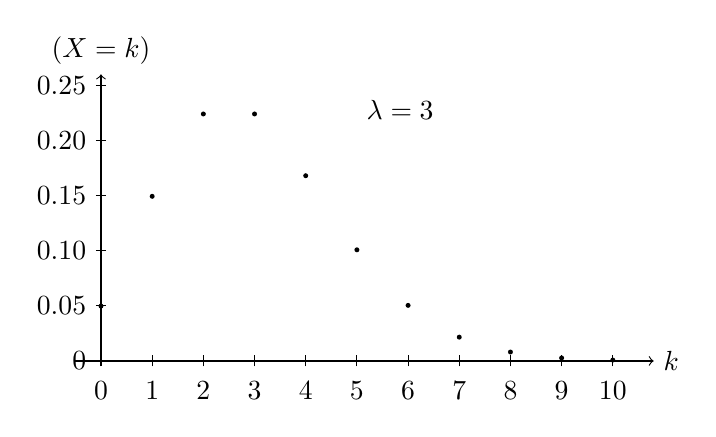
\begin{tikzpicture}[x=0.65cm,y=14cm]
    \draw[->] (-0.5,0) -- (10.8,0) node[right] {$k$};
    \draw[->] (0,0) -- (0,0.26) node[above] {$\bP(X=k)$};
    
    % y轴刻度标注
    \foreach \y in {0, 0.05, 0.10, 0.15, 0.20, 0.25} {
        \draw (-0.1,\y) -- (0.1,\y);
        \node[left] at (-0.1,\y) {\y};
    }
    
    % x轴刻度标注
    \foreach \x in {0, 1, 2, 3, 4, 5, 6, 7, 8, 9, 10} {
        \draw (\x,-0.005) -- (\x,0.005);
        \node[below] at (\x,-0.01) {\x};
    }
    
    % \lambda=3 时, k=0..10 的 pmf 数值(避免 pgfmath 阶乘/幂运算溢出)
    \foreach \kv/\pv in {
        0/0.04979,
        1/0.14936,
        2/0.22404,
        3/0.22404,
        4/0.16803,
        5/0.10082,
        6/0.05041,
        7/0.02160,
        8/0.00810,
        9/0.00270,
        10/0.00081
    } {
        \fill (\kv,\pv) circle (0.9pt);
    }
    \node[above right] at (5,0.21) {$\lambda=3$};
\end{tikzpicture}
\end{center}
\begin{remark}
当 \(n\to\infty\) 时, 
\(\text{Bin}(n, \lambda/n)\) 的 distribution 
趋近于 \(\text{Poi}(\lambda)\).\\
考虑 $X \sim B\left(n, \frac{\lambda}{n}\right)$, 对于固定的 $k$:
$$
\bP(X=k)=\binom{n}{k}\left(\frac{\lambda}{n}\right)^k\left(1-\frac{\lambda}{n}\right)^{n-k}
$$
展开组合数 $\binom{n}{k}$:
$$
\bP(X=k)=\frac{n(n-1) \ldots(n-k+1)}{k!} \cdot \frac{\lambda^k}{n^k} \cdot\left(1-\frac{\lambda}{n}\right)^n \cdot\left(1-\frac{\lambda}{n}\right)^{-k}
$$
重组项:
$$
\bP(X=k)=\frac{\lambda^k}{k!} \cdot \underbrace{\frac{n(n-1) \ldots(n-k+1)}{n^k}}_{(1)} \cdot \underbrace{\left(1-\frac{\lambda}{n}\right)^n}_{(2)} \cdot \underbrace{\left(1-\frac{\lambda}{n}\right)^{-k}}_{(3)}
$$
其中, (1) 的 limit 是 1, 
(2) 的 limit 是 $e^{-\lambda}$, (3) 的 limit 是 1, 因而 
\[
\lim_{n\to\infty} \mathbb{P}(X=k)= e^{-\lambda} \frac{\lambda^k}{k!}
\]
这个极限行为的意义是:
\begin{itemize}
    \item \(\lambda \) 表示: 在一个固定时间/空间窗口内, 一个事件出现的平均次数的观测.
    \item 我们把这段时间间分成 \(n\) 个小窗口, 将这个观测作为先验知识用来 model 这类事件实现的平均概率, 那么
     每个小窗口内事件出现的概率是 \(p = \lambda/n\).  
    \item 每个 \(\text{Bin}(n,\lambda / n)\) 都表示: 在时间细分成
     \(n\) 个小窗口的情况下, 这个事件出现的次数的分布. (注意不是在时间上的分布, 而是在次数上的分布)
    \item 当 \(n\to\infty\) 时, 其意义: 基于连续时间的估计, 
    这个事件在原固定事件窗口内出现的次数的分布. 这就是 
    \(\text{Poi}(\lambda)\) 的意义.
\end{itemize}
因而 Poisson distribution 的意义本质上是: 
\textbf{
给定对一个事件在固定窗口下出现的平均次数的观测(估计), 
那么这个事件在这个窗口内出现 \(n\) 次 
(\(n = 0,1,2,\cdots  \))的概率是多少?}\\
所以 Poisson 分布, 即是\textbf{根据一个事件在给定 windows 内发生次数的 expectation, 来估计这个事件在该 windows 内发生次数的分布的标准方法.}  \\
\end{remark}

\begin{remark}
Further remark: Poisson distribution 的用途.
\begin{itemize}
    \item 它是 model "大量级的小概率事件" 的通用模型.\\ 
    即一段时间内, 一件事情的发生的概率非常小 (\(p \ll 1\)), 
    但是有很多机会发生 (\(n \gg 1\)). 比如放射性衰变.
    \item 现实世界中, 对于一些事情, 我们想要 model 其在一段时间内发生的总次数 (\(n\)) 和单次成功率 (\(p\)) 
    是很困难的. 比如统计今天路过百货大楼的总人数 (\(n\)), 以及每个人路过百货大楼时走进去的概率 (\(p\)). 但是我们
    很容易可以知道: \(\lambda = np\) 的观测. 即: 每天平均有多少人走进百货大楼. 那么我们就可以用 Poisson distribution 来 model 这件事情在一天内发生的次数的分布.\\
\end{itemize}
\end{remark}
\end{example}






\section{continuous random variables}

\subsection{normal random variables}
(5.2 in book)
\begin{definition}
我们称 $X$ is \textbf{normally distributed with parameter $\mu$ and $\sigma$}, if the pdf of $X$ is given by: \[
\rho(x) = \frac{1}{\sigma \sqrt{2\pi}} e^{-\frac{(x - \mu)^2}{2 \sigma ^2}}
\]
写作: \[
X \sim \mathcal{N}(\mu, \sigma^2)
\]
\end{definition}
特别地, 当 $\mu =0, \sigma = 1$ 时, \[
X \sim \mathcal{N}(0, 1)
\]被称为 \textbf{standard normal distribution.}


容易验证: \(\int_{\mathbb{R}} \rho  = 1 \)

\[
I := \int_ 0^\infty e^{\frac{-y^2}{2}} \; dy
\]
\[
I^2 = \Bigg(\int_ 0^\infty e^{\frac{-y^2}{2}} \; dy\Bigg)\Bigg(\int_ 0^\infty e^{\frac{-x^2}{2}} \; dx\Bigg) = \int
\]






rescaling to std normal distribution: 
Suppose \[
Y \sim \mathcal{N}(\mu, \sigma^2)
\] we define \[
X : = \frac{Y - \mu}{\sigma}
\]
Then we have: \[
X \sim \mathcal{N}(0,1)
\]
这是容易验证的. 因为: \[
X \in B \;\; \Longleftrightarrow  \;\; \frac{Y-\mu}{\sigma} \in B \;\; \Longleftrightarrow  \;\; Y \in \sigma B + \mu
\]
因而 \[
P(X \in B ) = P(Y \in \sigma B + \mu)
\]






\subsection{expectation and variance of normal dist}
Suppose $ X \sim \mathcal{N}(0,1)$. Then \[
\mathbb{E}(X) =  \frac{1}{\sqrt{2\pi }} \int _{\mathbb{R}} x   e^{-\frac{x^2}{2}}    \; dx   = 0
\]
since this is \textbf{odd function}.

And  \begin{align}
    \mathbb{E}(X^2) &=  \frac{1}{\sqrt{2\pi }} \int _{\mathbb{R}} x^2   e^{-\frac{x^2}{2}}    \; dx   \\
    &= \frac{1}{\sqrt{2\pi }} \int _{\mathbb{R}} x (x  e^{-\frac{x^2}{2}})    \; dx \\
    &= \frac{1}{\sqrt{2\pi }} \int _{\mathbb{R}} x   ( e^{-\frac{x^2}{2}} )'   \; dx   \\
    & = - \frac{1}{\sqrt{2\pi }}  x e^{-\frac{x^2}{2}} \bigg|^\infty_{-\infty}  +  \frac{1}{\sqrt{2\pi }} \int _{\mathbb{R}}  e^{-\frac{x^2}{2}}    \; dx \\
    &= 0 + 1 = 1
\end{align}

从而: \[
Var(X) = 1
\]




For general normally distributed $Y$, 我们知道了 $X : = \frac{Y - \mu}{\sigma}$ 的 $\mathbb{E}(X)  = 0$, $Var(X) = 1$, 因而 \[
\mathbb{E}(Y) = \mathbb{E}(\sigma X + \mu)   = \mu
\]
\[
Var(Y)  = Var(\sigma X + \mu) =  \mathbb{E}[(\sigma X + \mu - \mu)^2] = \mathbb{E} (\sigma^2 X^2) = \sigma^2 \mathbb{E}[X^2] = \sigma^2 
\]

\begin{remark}
    对于 normally distributed $X$, 
    \[ \mathbb{E}(X^k) =  \frac{1}{\sqrt{2\pi}} \int_\mathbb{R} x^k  e^{-\frac{x^2}{2}}  \; dx  \]
    For $k$ odd, it is $0$.\\
    For $k$ even:
  \begin{align}
      \mathbb{E}(X^k) &=  \frac{1}{\sqrt{2\pi}} \int_\mathbb{R} x^{k-1} (x e^{-\frac{x^2}{2}})  \; dx  \\
      & = -\frac{1}{\sqrt{2\pi}} \int_\mathbb{R} x^{k-1} ( e^{-\frac{x^2}{2}}) ' \; dx \\
      &= 0 + \frac{1}{\sqrt{2\pi}} \int_\mathbb{R} (x^{k-1})' e^{-\frac{x^2}{2}} \;dx \\
      & = \frac{k-1}{\sqrt{2\pi}} \int_\mathbb{R} x^{k-2} e^{-\frac{x^2}{2}} \;dx  \\
      & = (k-1) \mathbb{E}(X^{k-2})
   \end{align}  
   从而: \[
   \mathbb{E(X^k )} = \begin{cases}
       0 ,\quad k = 2j-1 \\
       (2j-1)(2j-3)\cdots 1 = \frac{(2j)!}{2^j j!},\quad k=2j
   \end{cases}
   \]
\end{remark}




\subsection{cdf of normal distribution}
Let $X$ be the std normal distribution.\\
Its cdf given by: \[
\Phi(a) :=F_X(a)  = \int_{(-\infty,a]} \rho(x) \; dx = \frac{1}{\sqrt{2\pi}} \int_{(-\infty,a]}  e^{-\frac{x^2}{2}} \; dx
\]
Important numerical values:
\[
\Phi(-3) \approx 0.0013
\] 
\[
\Phi(-2) \approx 0.023
\]
\[
\Phi(-1) \approx 0.159
\]


Note 由于 $\rho$ (std) 是一个 even function, 有 \(P(X < -1) = P(X>1)\)
因而 \[
P(X \text{ is one std dev from mean}) = 2(P(X < -1)) = 2 \Phi(-1) \approx0.32 = 32\%
\]
Similarly, \[
P(X \text{ is two std dev from mean}) \approx 0.046 = 4.6\%
\]\[
P(X \text{ is three std dev from mean}) \approx 0.0026 = 0.26\%
\]

为什么 normal random variables 非常重要: comes from a "universality property" called \textbf{central limit theorem.} (will be covered later). Now we state a special case: 




Let $S_n$ be 投掷 $n$ 次 $p$-coin 中得到的 $\#$heads. 即 \[
P(H) := p
\]
我们已经知道, $S_n$ 是一个 binomial discrete random variable. 且有 \[
\mathbb{E}(S_n) = np, \quad  Var(S_n) = npq, \quad \sigma(S_n) = \sqrt{npq}
\]

 
\begin{theorem}{DeHavre's Central limit theorem}
    \[
    \lim_{n\to \infty} P\Bigg( \frac{S_n - \mathbb{E}(S_n)}{\sigma(S_n)} \in (a,b)\Bigg) = \Phi(b) - \Phi(a) = \frac{1}{\sqrt{2\pi}} \int_{(a,b)} e^{-\frac{x^2}{2}} \; dx
    \]
\end{theorem}




Write $S_n$ into $n$ 个 i.i.d. random variables
\[
S_n = \sum_{i=1}^n X_i
\]
each $X_i$ 都是一个 trial of tossing the $p$-coin.\\



\begin{example}
    Toss a million times 一个 fair coin. Approximate the prob that we get more than $501000$ heads: 
    \[
    \mathbb{E}(S_{1000000}) = np = 500000
    \]
    \[
    \sigma(S_{1000000}) = \sqrt{npq} = 500
    \] 因而: \[
    P(S_{1000000} > 501000) = P(S_{1000000} - \mathbb{E}(S_{1000000}) > 1000) = P(\frac{S_{1000000} - \mathbb{E}(S_{1000000})}{\sigma(S_{1000000})} > \frac{1000}{500}) = 1-\Phi(2) = \Phi(-2)  \approx 0.159  
    \]
\end{example}



(5.3 in book.)
\subsection{exponential random variables}

我们称 $X$ 为一个 exponential random variable with parameter $\lambda$, 如果它的 pdf is given by: \[
f(x) = \begin{cases}
    \lambda e^{-\lambda x}, \quad x > 0\\
    0, \quad x \leq 0
\end{cases}
\]


Distribution function given by: \[
F_X(x) = \begin{cases}
    \int _{-\infty}^x f(t) \; dt = \lambda \int_0 ^x e^{-\lambda t} \; dt = 1 - e^{-\lambda x}, \quad x> 0\\
    0,\quad x<0
\end{cases}
\]
容易验证, $F_X(x) =0$ when $x \to -\infty$, 以及 $F_X(x) \to 1$ when $x \to \infty$

\begin{align}
P(X> 0)& = 1 - P(X<0)      \\
&= 1- F_X(a) \\
&= e^{-\lambda a}
\end{align}


Expectation and moments: 
We compute the moment $\mathbb{E}[X^n], \quad n\geq 0$

$\mathbb{E}[X^0] = \mathbb{E}[1] = 1$

\begin{align}
\mathbb{E}[X^n] &= \lambda \int_0^\infty x^n e^{-\lambda x } \; dx  \\
&= - \int_0 ^\infty  x^n(e^{-\lambda x})' \; dx \\
&=  0 + \int_0 ^\infty n x^{n-1} e^{-\lambda x} \; dx \\
&= \frac{n}{\lambda} \mathbb{E}(X^{n-1})
\end{align}

因而 recursively get: \[
\mathbb{E}[X^n] = \frac{n!}{\lambda^n}
\]

\(\mathbb{E}[X] = \frac{1}{\lambda}, \mathbb{E}[X^2] = \frac{2}{\lambda^2}, \cdots  \)


从而: \[
Var[X] = \frac{2}{\lambda^2} - \frac{1}{\lambda^2} = \frac{1}{\lambda^2}
\]


Recall the Gamma function: \[
n!  = \int_0^\infty x^n e^{-x} \; dx  = \Gamma(n+1) \]


Interpretation: \textbf{exponential r.v. 是 geometric r.v. 的 continuous analogue.}


First time to get heads in a seq of Bernoulli coins:
\begin{align}
    p(k) &= (1-p)^{k-1} p  \\
    &= (1-p)^k \frac{p}{1-p}
\end{align}
如果我们令 $e^{-\lambda} := 1-p$
就得到: \[
p(k) = e^{-\lambda k} \frac{p}{1-p} 
\]
和 discrete 的 geometric distribution 相似, exponential distribution 是用来 \textbf{model the first time an event occurs}.


\begin{example}
    Suppose 一个 storage battery 的 lifetime 是 exponentially distributed 的, 并且 average 为 10 hours. Suppose 我们想要 use this battery for 5 hours for.
计算: probability of finishing the task, if:\\ 
(a) 使用一个 new battery\\
(b) 使用一个已经用过 2 hours 的 battery\\
\begin{solution}
    \[
    \mathbb{E}[X] = 10 = \frac{1}{\lambda} \implies \lambda = \frac{1}{10}
    \]
如果我们使用一个 new battery, 则 want: $P(X>5) = 1 - P(X<5) = 1- F_X(5) = e^{-\frac{1}{2}}$
如果我们使用一个用过 2 hours 的 battery, 则 want: \[
P(X> 5+2 \mid X > 2) = \frac{e^{-(5+2)\lambda}}{e^{-2\lambda }} = e^{-5\lambda} = = e^{-\frac{1}{2}}
\]
\end{solution}

Notice: 我们发现 \[
P(X>5) = P(X> 5+2 \mid X > 2)
\]
\end{example}

\begin{theorem}
一 ctn r.v. 有: \[
    P(X > b+ t \mid X > b) = P(X>t)
    \]
\textbf{当且仅当它是一个 exponential random variable.}
\end{theorem}
\begin{remark}
    "如果 $X$ 表示某个 event 发生的时间, 在已经过去时间 $b$ 而没发生的情况下, 再过时间 $t$ 发生这个时间的条件概率, 等于从时间 $0$ 开始, 过时间 $t$ 发生这个事件的初始概率."\\
    并且 notice 这是一个 iff statement
\end{remark}

\begin{proof}
\begin{align}
     &   P(X > b+ t \mid X > b) = P(X>t) \\
   \Longleftrightarrow  & P(X > b+t) = P(X > t) P(X>b) \\
    \Longleftrightarrow  & X \text{ exponential (check) }
\end{align}
\end{proof}





\subsection{Gamma distribution}

\begin{definition}{$\Gamma$-distribution}
Recall $\Gamma$ function: \[
    \Gamma(\alpha) = \int_0^\infty x^{\alpha - 1} e^{-x}\; dx
    \]
一个 ctn r.v. 被称为 have Gamma distribution with parameter $\alpha, \lambda$, 写作 $X \sim \Gamma(\alpha, \lambda)$, (其中 $\alpha > 0, \lambda > 0$), 如果它的 pdf 为 \[
f(x) = \begin{cases}
    \frac{\lambda e^{-\lambda x} (\lambda x)^{\alpha -1} }{\Gamma (\alpha)}, \quad x>0 \\
    0, \quad x \leq 0
\end{cases}
\]
\end{definition}
\begin{remark}
我们已经知道, $\Gamma$ 函数是对 define 在自然数上的 factorial 函数, 推广到 defined 在 $[0,\infty)$ 上.
我们有:  \[
\Gamma(\alpha + 1) = \alpha \Gamma(\alpha)
\]\[
n! = \Gamma(n+1)
\]
\end{remark}


Interpretation: $\Gamma$ distribution 的 random variable 是 binomial random variable 的 ctn version.

考虑 $\alpha : = n$ 为一个正整数, 那么它可以用来 model the first time an event occurs in a Poission process.

Expectation:  \begin{align}
    \mathbb{E}[X] &= \frac{1}{\Gamma(\alpha)} \int_0^\infty (\lambda x )^{\alpha -1} \lambda  e^{-\lambda x} \; dx\\
    &=  \frac{1}{\lambda \Gamma(\alpha)}  \int_0^\infty x^\alpha e^{-x} \; dx \\
    &= \frac{\Gamma(\alpha + 1)}{\lambda \Gamma(\alpha)} = \frac{\alpha}{\lambda}
\end{align}
(since $\Gamma(\alpha + 1) = \alpha \Gamma(\alpha)$.)

我们可以计算得: \[
\mathbb{E}[X^2] = \frac{\alpha}{\lambda^2}
\]

\subsection{Cauchy distribution}
\begin{definition}
    一个 random variable 被称为 have Cauchy distribution with parameter $\theta \in \mathbb{R}$, 如果它的 pdf 是: \[
    f(x)   =\frac{1}{\pi} \frac{1}{1+(x-\theta)^2} , \quad x\in \mathbb{R}
    \]
    当 $\theta = 0$ 时, 被称为 standard Cauchy distribution.
\end{definition}


CDF: \begin{align}
    F_X(a) = \int_{-\infty}^a f(x) \; dx &= \frac{1}{\pi} \int_0^\infty \frac{1}{1+ (x-\theta)^2} \; dx \\ 
    &= \frac{1}{\pi} \int_0^\infty  \frac{1}{1+ y^2} \; dy \\
    &= \frac{1}{\pi} \arctan y \Big|_{\infty}^{a - \theta} \\
    &=  \frac{1}{\pi} (\arctan (a - \theta) + \frac{\pi}{2}) \\
    &= \frac{1}{\pi} \arctan (a - \theta) + \frac{1}{2}
\end{align}

\begin{example}
A macro-beam flashlight is spin around tis center located at $(0,1)$.\\
假设 the angle of the flashlight is uniform in $(-\frac{\pi}{2}, \frac{\pi}{2})$, 并令 $X$ 为 the point on $x$-axis where the beam hits.\\
The distribution function of $X$ is: \[
F_X(a) = P(X < a) = P(\tan \alpha < a) = P(\alpha < \arctan a)
\]
因而 $X$ 为一个 std Cauchy r.v.  
\end{example}

Interpretation: Brownian motion models (among many other things) the motion of small particles, 比如气体和液体分子.\\

FACT: 如果 start the Brownian motion at $(0,1)$, 并令 $X $ 表示 the first point that the motion hits the $x$-axis, 那么 $X$ 为一个 std Cauchy r.v.  




\begin{remark}
Distribution of a function of a random variable: \\
令 $F_X$ 为一个 r.v. $X$ 的 cdf.\\
考虑 $Y := X^3$.\\
那么 $Y$ 的 distribution 是什么? \[
F_Y(a) = P(X^3 < a ) = P(X < a^3) = F_X(a^{1/3})
\]
更加 generally, 如果 \[
Y: = g(X)
\]
where $g$ 是一个 $\mathbb{R}\to \mathbb{R}$ 的 measurable function. \\
那么: \[
F_Y(a) = P(g(x) < a) = F_X(g^{-1} (a) )
\]
并且 pdf of $Y$: 
\begin{align}
\rho_y(x)  = \frac{d}{ dx} F_y(x) &= \frac{d}{dx} F_X(g^{-1}(a)) \\
&= F_X(g^{-1}(x)) \frac{d}{dx} g^{-1}(x) \\
&= f_x(g^{-1}(x)) \frac{d}{dx} g^{-1}(x)
\end{align}

\end{remark}












\section{independence}


